\chapter{Metric learning on subspace}
Euclidean is the most used metric, however, it can't measure the similarity of 


\section{Mahalanobis distance}
The Mahalanobis distance \cite{Mahadist} based metric learning has received much attention in similarity computing. The Mahanalobis distance of two observations $\bm{x} $ and $\bm{y}$ is defined as
\begin{equation}
D(\bm{x},\bm{y}) = (\bm{x} - \bm{y})^T\bm{M}(\bm{x} - \bm{y}), 
\end{equation}
where $\bm{x}$ and $\bm{y} $ are $d\times1$ observation vectors, $\bm{M}$ is a semi-positive definite matrix. Since $\bm{M}$ is semi-positive definite matrix, $\bm{M}$ can be decomposed as $\bm{M} = \bm{W}^T\bm{W}$, and Mahanalobis distance can also be written as 
\begin{equation}
D(\bm{x},\bm{y}) = (\bm{x} - \bm{y})^T\bm{W}^T\bm{W}(\bm{x} - \bm{y})= ||\bm{W}(\bm{x} - \bm{y})||
\end{equation}
 Therefore, Mahanalobis distance can be regarded as a variant of Euclidean distance.
 
 \section{Gradient descent optimization}
 Given a multivariate function $F(\bm{x})$, $\bm{x}$ is a $d$ dimensional vector, if $f(\bm{x})$ is continuous and differentiable in the neighbour of point $\bm{x}$ for all $\bm{x}$, then $f(\bm{x})$ decreases fastest in the direction of negative gradient of $F$ at $\bm{x}$. To compute the minimum of $F(\bm{x})$, an iterative method can be used by updating $F$ with respect to $\bm{x}$. If the updating step $\lambda$ is small enough, by updating $\bm{x}$ with 
 \begin{equation}
 \bm{x}_{t+1} = \bm{x}_{t} - \lambda \bm{G}
 \end{equation}
we have 
  \begin{equation}
 F(\bm{x}_{t+1}) \ge F(\bm{x}_t).
  \end{equation}
This process is repeated until certain condition is met, generally when gradient $||\bm{G}|| \le \eta$, $\eta$ is a very small positive integer. 
\begin{figure}
\centering
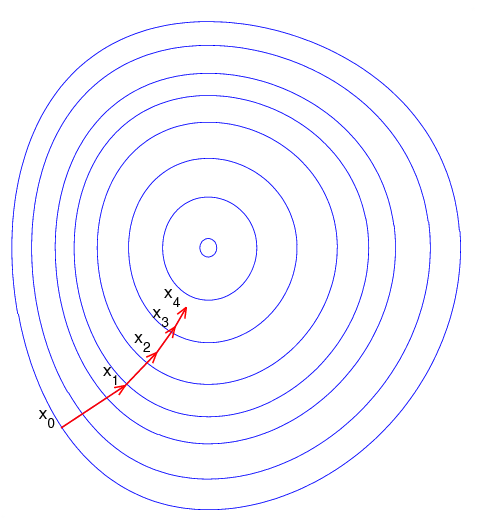
\includegraphics[width=0.4\linewidth]{/Users/JohnsonJohnson/Downloads/thesis_1/Figures/Gradientdescent.png}
\caption{Steepest gradient descent}
\vspace{0em}
\end{figure} 

\textbf{Analysis of steepest gradient descent method} The advantages of gradient descent are it's always downhill and it can avoid the saddle points. Besides, it's very efficient when initial value of $F(\bm{x})$ is further from minimum. However, there are a few shortcomings of gradient descent method. The first one is the convergence value of gradient descent might be the local minima of $F(\bm{x})$ if $F(\bm{x})$ is not monotonic \ref{fig:side:a}. In this case the convergence value will depend on the initial value of $\bm{x}$. Another shortcoming is the converging speed goes very slow when approaching the minimum. One example of slow approaching speed is the zigzag approaching case in figure \ref{fig:side:b}. The third shortcoming is linear search in gradient descent might cause some problem.
\begin{figure}[H]
\begin{minipage}[t]{0.5\linewidth}
\centering
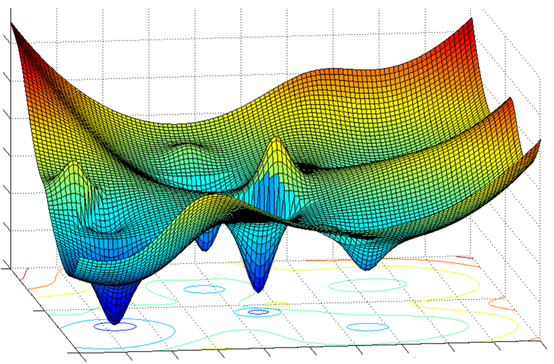
\includegraphics[width=2.2in]{/Users/JohnsonJohnson/Downloads/thesis_1/Figures/multiMinima.png}
\caption{Function with multi local minimums}
\label{fig:side:a}
\end{minipage}%
\begin{minipage}[t]{0.5\linewidth}
\centering
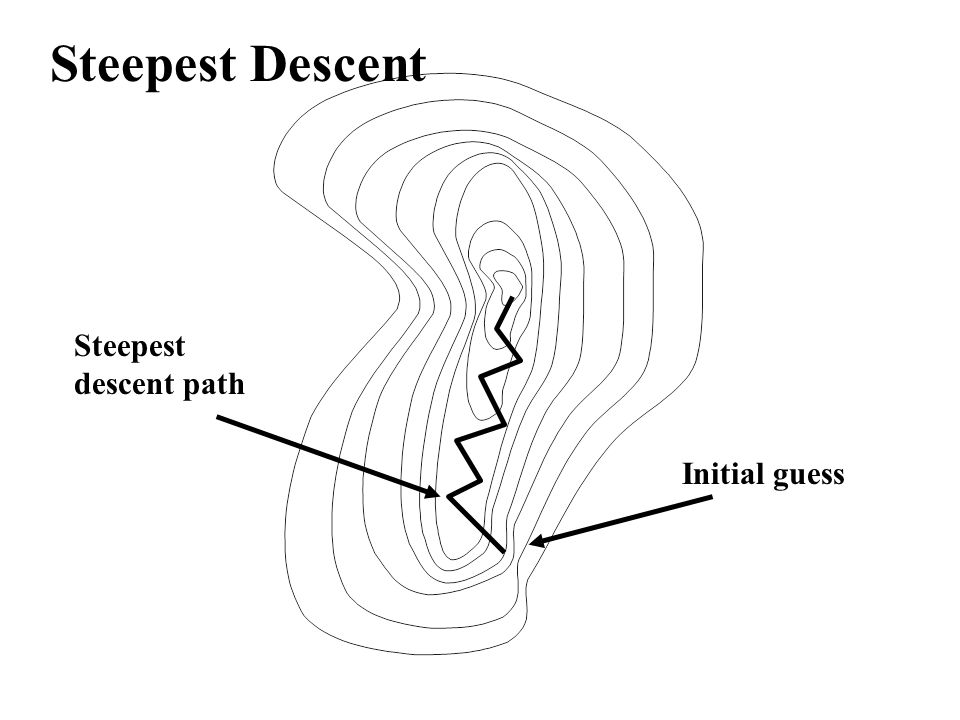
\includegraphics[width=2.2in]{/Users/JohnsonJohnson/Downloads/thesis_1/Figures/zigzag.jpg}
\caption{Zigzagging downhill valley}
\label{fig:side:b}
\end{minipage}
\end{figure}

 \section{Metric learning based on sample pairs distance comparison}
 Inspired by \cite{TDL}, in this paper, a similar metric learning based on iteration computation is used. For a  sample descriptor $\bm{x}_i$,  its positive pairwise set is defined as $\{\bm{x}_i,\bm{x}_j\}$, where class ID $y_i = y_j$. Also the negative pairwise set can be defined as $\{\bm{x}_i,\bm{x}_j\}$, where $y_i \ne y_j$. Similar with \cite{PRDC}, this method is also based on similarity comparison. The difference is in \cite{PRDC}, for all possible positive and negative pairs, the distance between positive pairs must be smaller than the distance between negative pairs. Since it has to compare all possible positive and negative pairs, its computation complexity is quite expensive. To decrease complexity, a simplified version is proposed as the top-push distance metric learning \cite{TDL}.  Since re-identification is a problem of ranking, it is desired that the rank-1 descriptor should be the right match. Given a Mahanalobis matrix $\bm{M}$, for samples $\bm{x}_i, i = 1,2,3,\cdots,n$, $n$ is the number of all samples, the requirement is distance between positive pair should be at least 1 unit smaller than the minimum distance of all negative pair. This can be denoted as 
 \begin{equation}
 D(\bm{x}_i,\bm{x}_j) + \rho < \min D(\bm{x}_i,\bm{x}_k), y_i = y_j, y_i\ne y_k.
 \end{equation}
 $\rho$ is a slack variable and $\rho \in [0,1]$. This equation can be transformed into a optimization problem as
 \begin{equation}
 \label{term1}
 \min \sum_{y_i = y_j} \max \{D(\bm{x}_i,\bm{x}_j) -  \min_{ y_i\ne y_k} D(\bm{x}_i,\bm{x}_k)  + \rho , 0\}.
 \end{equation}
However, the equation above only penalizes the minimum interclass distance. Another term is needed to penalize large intraclass distance. That is, the sum of intraclass distance should be as small as possible. This term is denoted as 
 \begin{equation} \label{term2}
 \min \sum_{y_i = y_j} D(\bm{x}_i,\bm{x}_j).
 \end{equation}

 
 To combine equations above, a ratio factor $\alpha$ is assigned to equation \eqref{term1} and \eqref{term2} so that the target function can be denoted as 
  \begin{equation}
  \begin{aligned}
 f(\bm{M}) = (1-\alpha)\sum_{\bm{x}_i,x_j,\bm{y}_i=y_j} D(\bm{x}_i,\bm{x}_j) + \\
  \alpha \sum_{\bm{x}_i,\bm{x}_j,y_i=y_j}\max\{{D(\bm{x}_i,\bm{x}_j)-\min_{y_i\ne y_k}{D(\bm{x}_i,\bm{x}_k)}+\rho,0}\}
 \end{aligned}
 \end{equation}
 In this way the problem is transformed to an optimization problem. Notice that equation 16 can be denoted as 
 \begin{equation}
 D(\bm{x},\bm{y}) = (\bm{x} - \bm{y})^T\bm{M}(\bm{x} - \bm{y}) = trace(\bm{M}\bm{X}_{i,j})
 \end{equation}
 where $\bm{X}_{i,j} = \bm{x}_i*\bm{x}_j^T$, and $trace$ is to compute matrix trace. Therefore, equation 21 can be transformed as follow,
 \begin{equation}
 \begin{aligned}
 f(\bm{M}) = (1-\alpha)\sum_{y_i = y_j}trace(\bm{M}\bm{X}_{i,j}) \\
  + \alpha \sum_{y_i = y_j,y_i\ne y_k}\max\{trace(\bm{M}\bm{X}_{i,j}) - trace(\bm{M}\bm{X}_{i,k} )+ \rho,0\}
 \end{aligned}
 \end{equation}
 
 To minimize equation 23, the gradient descent method is used. The gradient respect to $\bm{M}$ is computed as
 \begin{equation}
 \begin{aligned}
\bm{G} =  \frac{\partial f}{\partial \bm{M}} = (1-\alpha) \sum_{y_i = y_j} \bm{X}_{i,j} 
 + \alpha \sum_{y_i = y_j, y_i \ne y_k}(\bm{X}_{i,j} - \bm{X}_{i,k})
 \end{aligned}
 \end{equation}
 
 The iteration process can be summarized as in table \ref{Gradientdemo} 
% \begin{table}[H]
% \caption{The optimization algorithm for metric learning}
% \centering
% \begin{tabular}{l}
% \hline 
% \multicolumn{1}{l}{\textbf{Gradient optimization algorithm for target function}} \\
% \hline
% \textbf{Input} Descriptors of training person pairs \\
% \textbf{Output} A SPD matrix\\
% \textbf{Initialization} \\
% Initialize $\bm{M}$ with eye matrix $\bm{I}$; \\
% Compute the initial target function value $f_0$ with $\bm{M}_0$;\\
% Iteration count  $t = 0$;\\
%
% \textbf{while}(not converge)\\
% \space Update $t =  t + 1$;\\
% \indent Update gradient $\bm{G}_{t+1}$ with equation 24;\\
% \indent Update $\bm{M}$ with equation : $\bm{M}_{t+1} = \bm{M}_{t} - \lambda\bm{G}_t$\\
% \indent Project $\bm{M}_{t+1}$ to the positive semi-definite space \\ 
% \indent \indent by $\bm{M}_{t+1}= \bm{V}_{t+1}\bm{S}_{t+1}\bm{V}^T_{t+1}$;\\
% \indent Update the target value $f|_{\bm{M} = \bm{M}_{t+1}}$;\\
% \textbf{end while}  \\
% return $\bm{M}$\\
% \hline
% \end{tabular} 
% \end{table}
\begin{table}[H]
 \centering
 \caption{Optimization algorithm of Mahanalobis distance matrix learning}
 \begin{tabular}{l}
 \hline 
 \multicolumn{1}{l}{\textbf{Gradient optimization algorithm for target function}} \\
 \hline
 \textbf{Input} Descriptors of training person pairs \\
 \textbf{Output} A SPD matrix\\
 \textbf{Initialization} \\
 Initialize $\bm{M}_0$ with eye matrix $\bm{I}$; \\
 Compute the initial target function value $f_0$ with $\bm{M}_0$;\\
 Iteration count  $t = 0$;\\

 \textbf{while}(not converge)\\
 \indent Update $t =  t + 1$;\\
 \indent Find $\bm{x}_k$ for all sample points $\bm{x}_i$, where $y_i \ne y_k$;\\
 \indent Update gradient $\bm{G}_{t+1}$ with equation 12;\\
 \indent Update $\bm{M}$ with equation : $\bm{M}_{t+1} = \bm{M}_{t} - \lambda\bm{G}_t$;\\
 \indent Project $\bm{M}_{t+1}$ to the positive semi-positive definite space; \\ 
% \indent \indent by $\bm{M}_{t+1}= \bm{V}_{t+1}\bm{S}_{t+1}\bm{V}^T_{t+1}$;\\
 \indent Update the target value $f|_{\bm{M} = \bm{M}_{t+1}}$;\\
 \textbf{end while}  \\
 return $\bm{M}$\\
 \hline
 \end{tabular} 
 \end{table}
 \label{Gradientdemo}
In each iteration, to make sure the updated $\bm{M}$ is a SPD matrix, first a eigenvalue decomposition is performed on $\bm{M}$, and we have
\begin{equation}\label{SPDproject}
\bm{M} = \bm{V}\bm{\Lambda}\bm{V}^T
\end{equation}
Then the negative eigenvalues in $\bm{V}$ are removed and the corresponding eigenvectors in $\bm{V}$ are also removed. Then $\bm{M}$ is restored by equation \eqref{SPDproject}.

 
 
 
 
 
